\section{Planetary escape and capture}
\label{sec:stations}
For a station on a circular parking orbit, take its radius as the local
length scale. The station state is
$x_s(t)=e_r(\phi_s+t)$, $v_s(t)=e_\theta(\phi_s+t)$.
Escape starts at that state and ends at the first outward SOI crossing.
Capture starts at an inward crossing and must match both station
position and velocity at the actual arrival epoch.
Matching the orbital radius alone is insufficient.

\subsection{A solvable circular approximation}
For a slowly evolving circular orbit let $q=r^{-1/2}$.
Tangential acceleration gives the leading-order equations
\begin{equation}
 q'=-a_t,\qquad \theta'=q^3,\qquad r'=2r^{3/2}a_t.
 \label{eq:spiral}
\end{equation}
The validity diagnostic is
$\eta_{\rm ad}=|a_t|r^2\ll1$; the radial-to-circular-speed ratio
is $2\eta_{\rm ad}$. This approximation assigns radial drift during a
burn and cannot be attached literally to an exactly circular initial
state with zero radial speed.

Assume monotone radius and free phase, put $D=|q_i-q_f|$ and
$a=|a_t|$. Then $\int a\,dt=D$. The ideal minimum effort is $D^2/h$,
attained by constant $a=D/h$. For the finite band, $w'=a^2$ and
the final inverse mass is $W=\chi+J$.
On powered intervals use $z=1/a$ and $w$ as the independent variable:
\begin{equation}
 \begin{gathered}
 \int_\chi^W z\,dw=D,\qquad T_b=\int_\chi^W z^2\,dw,\\
 \nu_-/w\le z\le\nu_+/w.
 \end{gathered}
\end{equation}
Coasts consume neither progress nor mass in this model.

\begin{proposition}[Finite-band circular profile]
For fixed $W$ and feasible monotone progress $D$, the unique
minimum-burn-time profile almost everywhere is
\begin{equation}
 z_*(w)=\operatorname{clip}(k,\nu_-/w,\nu_+/w),\qquad
 \int_\chi^W z_*\,dw=D,
 \label{eq:spiralsolution}
\end{equation}
where feasibility is
$\nu_-\log(W/\chi)\le D\le\nu_+\log(W/\chi)$.
\end{proposition}
\begin{proof}
For a fixed scalar $k$, pointwise projection minimizes $(z-k)^2$
on the interval. Integrating and comparing any other feasible $z$,
the equality of $\int z\,dw$ cancels the linear term, leaving
$\int z_*^2dw\le\int z^2dw$. Strict convexity gives uniqueness.
The integral of the clipped profile is continuous and monotone in $k$.
\end{proof}

As $w$ increases the profile uses, when present, minimum exhaust,
constant acceleration and maximum exhaust. This ordering is specific
to the reduced model. Define
\begin{equation}
 \begin{gathered}
 w_1=\operatorname{clip}(\nu_-/k,\chi,W),\\
 w_2=\operatorname{clip}(\nu_+/k,w_1,W).
 \end{gathered}
\end{equation}
The scalar root uses the elementary formulas
\begin{equation}
 \begin{split}
 D={}&\nu_-\log(w_1/\chi)+k(w_2-w_1)
                 +\nu_+\log(W/w_2),\\
 T_b={}&\nu_-^2(\chi^{-1}-w_1^{-1})+k^2(w_2-w_1)\\
       &+\nu_+^2(w_2^{-1}-W^{-1}).
 \end{split}
 \label{eq:spiralintegrals}
\end{equation}
For constant exhaust $\nu$,
\begin{equation}
 J_\nu=\chi(e^{D/\nu}-1),\qquad
 T_\nu=\frac{\nu^2}{\chi}(1-e^{-D/\nu}).
\end{equation}
Set $T_{\rm fast}=T_{\nu_-}$ and $T_{\rm slow}=T_{\nu_+}$.
For $D>0$, duration below $T_{\rm fast}$ is infeasible in the
reduced model. Between these times there is a unique effort giving
$T_b=h$; above $T_{\rm slow}$ the optimum is a maximum-exhaust burn
plus coast, with the positive floor $J_{\nu_+}$.
At fixed $D$, the interior envelope derivative of burn time with
respect to $W$ is $z_*(W)^2-2kz_*(W)<0$, establishing the outer
monotone effort root. For $D=0$, zero effort is sufficient when
phase is free.

\begin{figure}[tb]
\centering
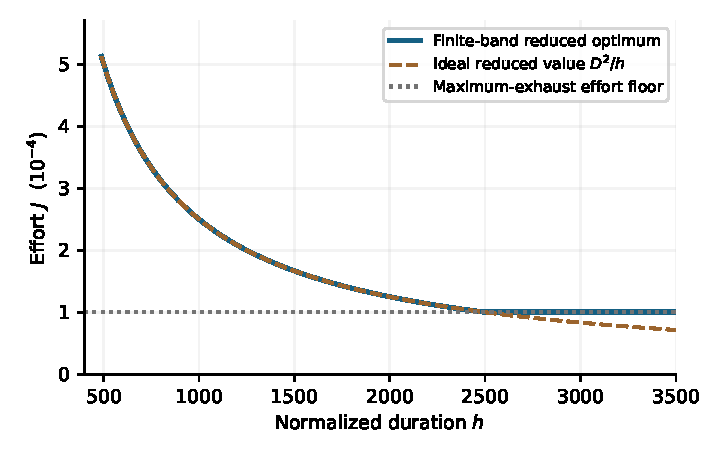
\includegraphics[width=\columnwidth]{figures/averaged_effort.pdf}
\caption{Minimum effort in the phase-free monotone circular model:
$D=0.5$, $\chi=0.01$, $\nu_-=10$, $\nu_+=50$.
The finite ceiling produces a long-duration fuel floor.}
\label{fig:spiral}
\end{figure}

Station phase adds a constraint. For constant acceleration the
accumulated angle is
\begin{equation}
 \Delta\theta=\frac h4(q_i^3+q_i^2q_f+q_iq_f^2+q_f^3).
\end{equation}
It is not a free output. On the maximum-exhaust plateau, let
$c=h-T_{\rm slow}$ and let $\Theta_b$ be the burn angle.
Placing coast at the initial and final radii gives exactly the range
\begin{equation}
 \Theta_b+c\min(q_i^3,q_f^3)
 \le\Delta\theta\le
 \Theta_b+c\max(q_i^3,q_f^3)
\end{equation}
at that minimum fuel, within the monotone approximation.
Outside this range phase costs additional effort or makes the chosen
duration infeasible. A fixed-phase ideal interior satisfies
$2q''=3\Lambda q^2$, rather than generally $q''=0$.

Neither reduced infeasibility nor its optimum is a full Kepler
certificate. Constant nonzero acceleration eventually makes
$|a_t|r^2$ large. For example, the earlier Earth illustration with
7000 km parking radius, chosen 900000 km SOI and useful
$P/m_0=540\,\mathrm{W/kg}$ gives an initial minimum powered
acceleration $0.00432\,\mathrm{m/s^2}$. Its slow-spiral diagnostic
already reaches $0.05$ near 67922 km from Earth's center.
The calculation is a validity warning for continuous slow spirals,
not a prediction of optimized Earth escape \cite{JPLParameters}.

\subsection{An exact feasible pair}
Exact analytic curves are useful independent tests of a controlled
Kepler solver \cite{PetropoulosSims2002}. In local units $\mu=1$, set
$0\le t\le10$ and
\begin{equation}
 \begin{gathered}
 r=1+0.03t^2,\qquad \theta=t/\sqrt r,\qquad \theta'=r^{-3/2},\\
 x=re_r,\quad v=0.06t\,e_r+r^{-1/2}e_\theta,\\
 u=0.06e_r+0.03t\,r^{-3/2}e_\theta.
 \end{gathered}
 \label{eq:exactescape}
\end{equation}
Direct differentiation gives $x''=-x/r^3+u$. It starts on the unit
circle, first reaches $r=4$ at $t=10$, and ends with
$\theta=5$, $v_r=0.6$, $v_t=0.5$, $E=0.055$.
The effort and a full-time acceleration enclosure are
\begin{equation}
 \begin{gathered}
 U=\frac{651}{16000}+\frac{\pi\sqrt3}{240}
 =0.0633599920529\ldots,\\
 0.06\le|u|\le\frac{\sqrt{181}}{150}<0.09.
 \end{gathered}
\end{equation}
With $\chi=0.9$, budget $0.08$, floor $0.8$ and band $[10,50]$,
$(\chi+U)/50<0.06$ and $\chi/10=0.09$.
Thus the curve is safe and band-feasible throughout, without relying
on sampling. It retains mass fraction $0.9342302020\ldots$.

Let $Q=\operatorname{diag}(1,-1)$. The reflected reversal
$x_c(t)=Qx(10-t)$, $v_c(t)=-Qv(10-t)$ and
$u_c(t)=Qu(10-t)$ preserves prograde angular momentum and arrives
at $(1,0,0,1)$. A unit station with initial phase $-10$ rendezvous
at this endpoint. The same magnitude enclosure proves band feasibility
for the same initial $\chi$, but the mass history is recomputed
forward: reversing position and velocity does not reverse fuel use.

\begin{figure}[tb]
\centering
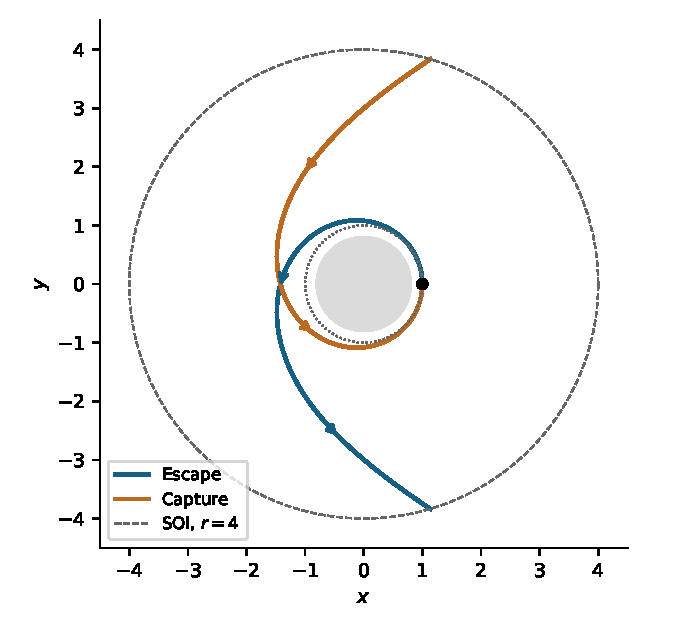
\includegraphics[width=\columnwidth]{figures/exact_escape_capture.pdf}
\caption{Exact escape and reflected capture examples. The station orbit
is dotted, the SOI is dashed, and $r<0.8$ is excluded.
These are separate feasible local trajectories.}
\label{fig:escape}
\end{figure}

For arbitrary endpoint energies in the annulus, define
$W_E=\sqrt{2E+2/\varepsilon}$. Since $|v|\le W_E$,
equation~\eqref{eq:work} gives $|W_E'|\le|u|$; also
$|j'|\le\sigma_S|u|$.
With $d_*=\max(|\Delta W_E|,|\Delta j|/\sigma_S)$, every
full-power/coast transfer satisfies
\begin{equation}
 J\ge
 \max\left\{\frac{d_*^2}{h},\
 \chi\left(e^{d_*/\nu_+}-1\right)\right\}.
 \label{eq:localbound}
\end{equation}
The second term follows from
$\int|u|dt\le\nu_+\log(1+J/\chi)$.
It remains valid for nonpositive $E$ whenever the endpoint states
are admissible.
For \eqref{eq:exactescape}, the energy part and feasible construction
give the symbolic same-endpoint bracket
\begin{equation}
 \frac{411-30\sqrt{174}}{1000}\le V_{\rm exact}\le
 \frac{651}{16000}+\frac{\pi\sqrt3}{240}.
 \label{eq:exactbracket}
\end{equation}
This establishes a feasible upper bound and a global lower bound in
the stated patch model; the constructed curve is not asserted stationary.
